\section{Regression}
For the first half of this assignemnt we will try an use regression to predict the "refractive index - RI" of the glass given the chemical components contained in our dataset.\\
We will start of by just doing forward feature selection using k-fold cross-validation, such that we get the best variables for our linear regression, and reduce the chance of our model overfitting.\\
\begin{figure}
    \centering
    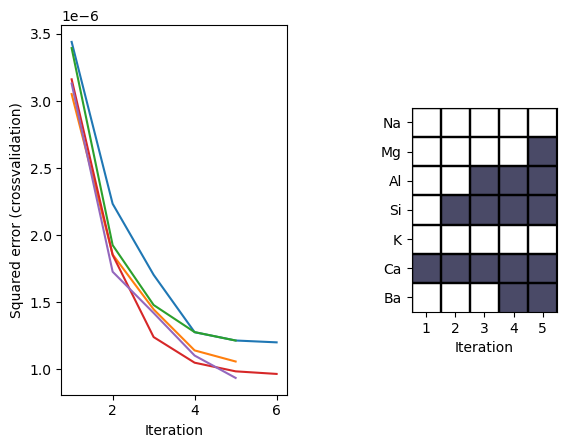
\includegraphics[width=12cm]{images/featureselection.png}
    \caption{Feature selection}
    \label{fig:fig_select}
\end{figure}
As such we are left we 2 less variables and can reduce the dimensionality of our dataset from the get-go. \\

Next we standardize the full dataset such that the mean of all the variable is 0 and the standard deviation is 1. \color[red]{It is worth noting that the helper function "rlr_validate" also standardizes its internal data partitions as a part of kfold cross-validation when it selects values of $\lambda$} \\
To the further prevent overfitting we introduce a regularization parameter $\lambda$, which we determine by testing different values and evaluate using the generalization error